\pdfminorversion=4
\documentclass[9pt]{beamer}
\usepackage[utf8]{inputenc}
\usepackage[T1]{fontenc}
\usepackage{adjustbox}
\usepackage{graphicx}
\usetheme{urcatex}
\usepackage{algorithm,algorithmic}

\newcommand \ve[1]{\mathbf{#1}}
\title[Introduction aux réseaux de neurones]{Les réseaux de Neurones}


\author[F. Alin]{François Alin}

\AtBeginSection[]
{
  \begin{frame}<beamer>
    \frametitle{Sommaire}
{\tableofcontents[currentsection]
}
  \end{frame}
}

\begin{document}

\begin{frame}
	\titlepage
\end{frame}


\section*{Sommaire}
\begin{frame}
	\tableofcontents
\end{frame}

\section{Contexte}
\begin{frame}
\frametitle{Contexte}
\begin{block}{Big Data}
\begin{itemize}
\item Surabondance de données: images, vidéos, audio, texte, traces d'utilisation, etc;
\begin{center}
\includegraphics[scale=0.2]{images/fig1.png} 
\end{center}
\item Besoin évident d'accéder, de rechercher ou de classer ces données: Reconnaissance
\item Nombreuses applications: recherche visuelle mobile, robotique, conduite autonome,
réalité augmentée, imagerie médicale, etc.
\item Parcours de premier plan dans les principales conférences ML / CV au cours de la dernière décennie
\begin{center}
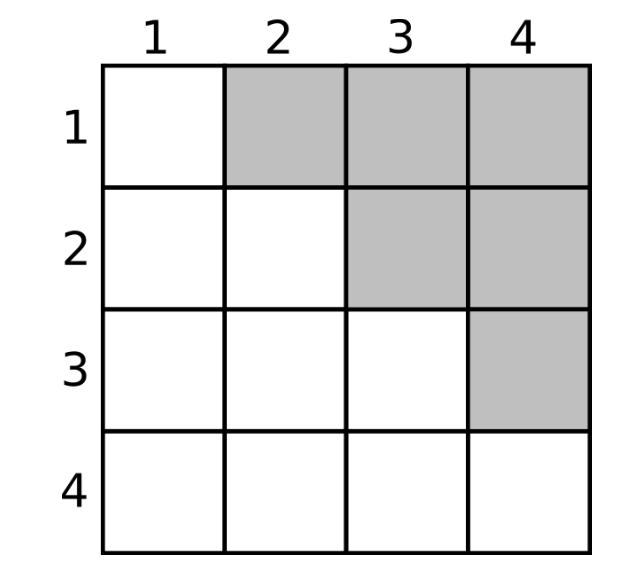
\includegraphics[scale=0.2]{images/fig2.png} 
\end{center}
\end{itemize}
\end{block}
\end{frame}

\begin{frame}
\frametitle{Reconnaissance et classification}
\begin{itemize}
\item Classification: attribuez une classe à un ensemble donné de classes prédéfinies 
\item La reconnaissance est beaucoup plus générale que la classification, par ex.
\begin{itemize}
\item Localisation d'objets d'objets images
\item Classement pour l'indexation de documents
\item Prédiction de séquence pour le texte, la parole, l'audio, etc.
\end{itemize}
\item Plusieurs tâches peuvent être transformées en problèmes de classification  $\Rightarrow$ importance de la classification
\end{itemize}
\begin{center}
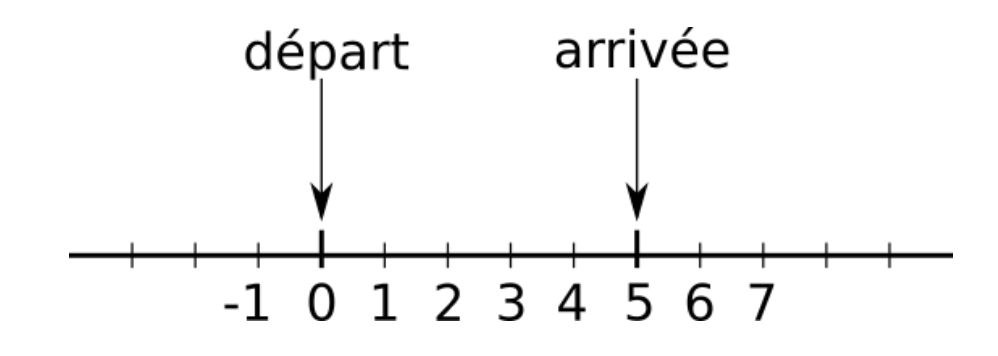
\includegraphics[scale=0.3]{images/fig3.png} 
\end{center}
\end{frame}

\begin{frame}
\frametitle{Focus sur la reconnaissance visuelle : Percevoir le monde Réel}
\begin{itemize}
\item Reconnaissance visuelle: archétype de la compréhension du signal de bas niveau 
\item Censé être un problème de classe maîtresse au début des années 80
\item Certainement le sujet le plus touché par l'apprentissage en profondeur
\end{itemize}

\begin{tabular}{lc}
\begin{minipage}{4cm}
Catégorisation de scène
\begin{itemize}
\item localisation d'objet
\item Reconnaissance du contexte et des attributs
\item Mise en page 3D approximative, classement des profondeurs
\item Description détaillée de la scène, par exemple phrases
\end{itemize}
\end{minipage}

 &
 
 \begin{minipage}{4cm}
\begin{center}
 \includegraphics[scale=0.2]{images/fig4.png}  
\end{center}
 \end{minipage}
\end{tabular}
\end{frame}

\begin{frame}
\frametitle{Reconnaissance de signal faible}

\begin{tabular}{ccc}

 \begin{minipage}{4cm}
\begin{center}
 \includegraphics[scale=0.25]{images/fig5.png}  
\end{center}
 \end{minipage}
&
\begin{minipage}{3cm}
Ce que nous voyons vs ce que voir l'ordinateur !! 
\end{minipage}
 &
 \begin{minipage}{4cm}
\begin{center}
 \includegraphics[scale=0.15]{images/fig6.png}  
\end{center}
 \end{minipage}
\end{tabular}

\begin{tabular}{cc}
 \begin{minipage}{6cm}

 \includegraphics[scale=0.2]{images/fig7.png}  

 \end{minipage}
 
&

\begin{minipage}{5cm}
\begin{itemize}
\item Variations d'éclairage 
\item Variations de points de vue 
\item Objets déformables
\item  variance intra-classe
\item etc
\end{itemize}
\end{minipage}
\end{tabular}
\begin{alertblock}{}
\begin{center}
Comment choisir une bonne représentation intermédiaire? 
\end{center}
\end{alertblock}
\end{frame}

\begin{frame}
\frametitle{Deep Learning et reconnaissance des signaux faibles}

\begin{itemize}
\item DL : une percée dans la reconnaissance des signaux faibles
\item Avant le DL : Construction manuelle de représentation intermédiaire pour chaque tâche
\begin{itemize}
\item Nécessité d'un expert dans chaque domaine;
\item Faible niveau sémantique de la représentation
\end{itemize}
\end{itemize}
\begin{center}
\includegraphics[scale=0.4]{images/fig8.png}
\end{center}

\end{frame}

\begin{frame}
\frametitle{Deep Learning et reconnaissance des signaux faibles}

\begin{itemize}
\item DL : une percée dans la reconnaissance des signaux faibles
\item Depuis le DL : Construction manuelle de représentation intermédiaire pour chaque tâche
\begin{itemize}
\item Des performances remarquables >> extracteurs manuels
\item Capable d'apprendre des représentations intermédiaires de haut niveau
\item Méthodologie d'apprentissage commune $\Rightarrow$ indépendante du domaine, pas de nécessité d'expertise
\end{itemize}
\end{itemize}
\begin{center}
\includegraphics[scale=0.4]{images/fig9.png}
\end{center}

\end{frame}

\begin{frame}
\frametitle{Deep Learning et modélisation des données}

\begin{itemize}
\item DL :  percée pour l'apprentissage de la représentation
\begin{itemize}
\item Apprentissage automatique des niveaux intermédiaires de représentation
\end{itemize}
\end{itemize}

\begin{minipage}[c]{0.5\linewidth}
\begin{itemize}
\item Ex: Traitement en langage naturel (NLP)
\end{itemize}
\includegraphics[scale=0.4]{images/fig10.png}
\end{minipage} \hfill
\begin{minipage}[c]{0.25\linewidth}
\includegraphics[scale=0.4]{images/fig11.png}
\end{minipage}
\end{frame}

\section{Réseau de Neurones}
\begin{frame}
\frametitle{Neurone formel : 1943}
\begin{itemize}
\item Base des réseaux de neurones;
\item Entrée : vecteur $\ve{x}\in\mathcal{R}^m$ càd $\ve{x}={x_i}_{i\in \{1,2,\cdots ,m\}}$
\item Sortie : $\hat{y}\in \mathcal{R}$ un scalaire.
\end{itemize}
\begin{center}
\includegraphics[scale=0.4]{images/fig12.png}
\end{center}
\end{frame}


\begin{frame}
\frametitle{Neurone formel : 1943}
\begin{itemize}
\item Relation entre $\ve{x}$ et $\hat{y}$ :
\begin{enumerate}
\item Relation linéaire (affine) : $s=\ve{w}^T\ve{x}+b$
\item Fonction d'activation non linéaire $f$ : $\hat{y}=f(s)$
\end{enumerate}
\end{itemize}
\begin{center}
\includegraphics[scale=0.4]{images/fig13.png}
\end{center}
\end{frame}

\begin{frame}
\frametitle{Neurone Formel : Transformation linéaire}
\begin{itemize}
\item Relation linéaire : $s=\ve{w}^T\ve{x}+b = \sum_{i=1}^m w_ix_i+b$
\begin{itemize}
\item $\ve{w}$ : vecteur normal à un hyperplan de $\mathcal{R}^m\Rightarrow$ frontière linéaire;
\item b biais, translation de l'hyperplan.
\end{itemize}
\end{itemize}
\vspace{1cm}
\includegraphics[scale=0.4]{images/fig14.png}
\end{frame}

\begin{frame}
\frametitle{Neurone formel : Fonction d'activation}
\begin{itemize}
\item $\hat{y} = f\left((\ve{w}^T\ve{x}+b\right)$, $f$ est appelée fonction d'activation;
\begin{itemize}
\item fonctions d'activation usuelles : échelon, sigmoid, tanh.
\end{itemize}
\item Fonction de Heaviside (échelon) : 
$
H(z)=
\begin{cases}
1 \text{ si } z\geqslant 0 \\
0 \text{ sinon}
\end{cases}
$
\end{itemize}
\includegraphics[scale=0.4]{images/fig15.png}
\end{frame}

\begin{frame}
\frametitle{Fonction d'activation : Similitude avec un neurone biologique}
\includegraphics[scale=0.25]{images/fig16.png}
\begin{itemize}
\item Neurone formel, fonction d'activation $H$ : $\hat{y}=H\left(\ve{w}^T\ve{x}+b\right)$
\begin{itemize}
\item $\hat{y} = 1$ (état activé) $\Leftrightarrow \ve{w}^T\ve{x}\geqslant -b$
\item $\hat{y} = 0$ (état désactivé) $\Leftrightarrow \ve{w}^T\ve{x}< -b$
\end{itemize}
\item Neurones biologiques : sortie active $\Leftrightarrow$ entrée pondérée par les poids synaptiques $\geqslant$ au seuil.
\end{itemize}
\end{frame}

\begin{frame}
\frametitle{Fonction sigmoïde}
\begin{itemize}
\item Sortie du neurone $\hat{y}=f\left(\ve{w}^T\ve{x}+b\right)$, $f$ fonction d'activation
\item Sigmoïde : $\sigma(z)=(1+e^{-az})^{-1}$
\begin{center}
\includegraphics[scale=0.3]{images/fig17.png}
\end{center}
\item $a\nearrow$ = tend vers la fonction échelon (echelon $a\rightarrow\infty$)
\item Sigmoïde : présence de régime linéaire et de régime de saturation.
\end{itemize}
\end{frame}

\begin{frame}
\frametitle{Neurone formel : Application à la classification binaire}
\begin{itemize}
\item Classification binaire : Le label d'entrée $\ve{x}$ doit appartenir à la classe 0 ou 1
\item Sortie dans le cas de la sigmoïde : $\hat{y}=\frac{1}{1+e^{-a\left(\ve{w}^T\ve{x}+b\right)}}$
\item Sigmoïde : interprétation probabiliste $\Rightarrow \hat{y}\sim P\left(1/\ve{x}\right)$
\begin{itemize}
\item Entrée $\ve{x}$ classifiée comme 1 si $P\left(1/ve{x}\right) > 0.5 \Leftrightarrow \ve{w}^T\ve{x}+b>0$
\item Entrée $\ve{x}$ classifiée comme 0 si $P\left(1/ve{x}\right) < 0.5 \Leftrightarrow \ve{w}^T\ve{x}+b<0$
\end{itemize}
\end{itemize}
\begin{center}
\includegraphics[scale=0.3]{images/fig18.png}
\end{center}
\begin{alertblock}{}
$\Rightarrow sign \left(\ve{w}^T\ve{x}+b\right)$ définit la frontière linéaire de décision dans l'espace d'entrée
\end{alertblock}
\end{frame}


\begin{frame}
\frametitle {Neurone formel : Exemple}

\begin{minipage}[c]{0.7\linewidth}
\begin{itemize}
\item Exemple 2D : $m=2$, $\ve{x}=\{x_1, x_2\}\in[-5,5]\times[-5,5]$
\item Transformation linéaire : $\ve{w}=[1,1]$ et $b=-2$
\item Sortie du réseau linéaire : $s=\ve{w}^T\ve{x}+b$
\end{itemize}
\end{minipage} \hfill
\begin{minipage}[l]{0.25\linewidth}
\includegraphics[scale=0.3]{images/fig19.png}
\end{minipage}
\begin{block}{
Fonction d'activation sigmoïde $\hat{y}=\left(1+e^-a{\left(\ve{w}^T\ve{x}+b\right)}\right)^{-1}$ avec $a=10$}

\begin{center}
\includegraphics[scale=0.3]{images/fig20.png}
\end{center}
\end{block}
\end{frame}

\begin{frame}
\frametitle {Neurone formel : Exemple}

\begin{minipage}[c]{0.7\linewidth}
\begin{itemize}
\item Exemple 2D : $m=2$, $\ve{x}=\{x_1, x_2\}\in[-5,5]\times[-5,5]$
\item Transformation linéaire : $\ve{w}=[1,1]$ et $b=-2$
\item Sortie du réseau linéaire : $s=\ve{w}^T\ve{x}+b$
\end{itemize}
\end{minipage} \hfill
\begin{minipage}[l]{0.25\linewidth}
\includegraphics[scale=0.3]{images/fig19.png}
\end{minipage}
\begin{block}{
Fonction d'activation sigmoïde $\hat{y}=\left(1+e^-a{\left(\ve{w}^T\ve{x}+b\right)}\right)^{-1}$ avec $a=1$}

\begin{center}
\includegraphics[scale=0.3]{images/fig21.png}
\end{center}
\end{block}
\end{frame}

\begin{frame}
\frametitle {Neurone formel : Exemple}

\begin{minipage}[c]{0.7\linewidth}
\begin{itemize}
\item Exemple 2D : $m=2$, $\ve{x}=\{x_1, x_2\}\in[-5,5]\times[-5,5]$
\item Transformation linéaire : $\ve{w}=[1,1]$ et $b=-2$
\item Sortie du réseau linéaire : $s=\ve{w}^T\ve{x}+b$
\end{itemize}
\end{minipage} \hfill
\begin{minipage}[l]{0.25\linewidth}
\includegraphics[scale=0.3]{images/fig19.png}
\end{minipage}
\begin{block}{
Fonction d'activation sigmoïde $\hat{y}=\left(1+e^-a{\left(\ve{w}^T\ve{x}+b\right)}\right)^{-1}$ avec $a=0.1$}

\begin{center}
\includegraphics[scale=0.3]{images/fig22.png}
\end{center}
\end{block}

\end{frame}

\begin{frame}
\frametitle{Du neurone formel au réseau de neurones}
\begin{minipage}[l]{0.5\linewidth}
\begin{itemize}
\item Neurone formel
\begin{enumerate}
\item Une sortie scalaire unique;
\item Frontière de décision linéaire pour classification binaire
\end{enumerate}
\item Sortie scalaire unique $\Rightarrow$ trop limité pour de nombreuses tâches
\begin{itemize}
\item classification multiclasses telle que MNIST ou CIFAR
\end{itemize} 
\end{itemize}
\end{minipage}
\begin{minipage}[c]{0.4\linewidth}
\includegraphics[scale=0.3]{images/fig23.png}
\end{minipage}

\begin{center}
\includegraphics[scale=0.3]{images/fig24.png}
\end{center}
\end{frame}

\begin{frame}
\frametitle{Perceptron et Classification multi-classe}
\begin{minipage}[c]{0.5\linewidth}
\begin{itemize}
\item Neurone formel : limité à la classification binaire
\item Classification multi-classe : Utilisation de plusieurs neurones au lieu d'un seul. $\Rightarrow$ \textbf{Perceptron}
\item Vecteur d'entrée $\ve{x}$ dans $\mathcal{R}^n$
\item Le neurone de sortie $\hat{y}_1$ est un neurone formel:
\begin{itemize}
\item Transformation affine : $s_1=\ve{w_1}^T\ve{x}+b_1$
\item Fonction d'activation non linéaire $f$ tq $\hat{y}_1=f(s_1)$
\end{itemize}
\item Paramètre de la transformation linéaire : 
\begin{itemize}
\item $\ve{w_1} = \left\lbrace w_{11}, \cdots ,w_{m1}\right\rbrace \in \mathcal{R}^m$
\item $b_1 \in \mathcal{R}$ 
\end{itemize}
\end{itemize}
\end{minipage}
\begin{minipage}[c]{0.4\linewidth}
\includegraphics[scale=0.25]{images/fig25.png}
\end{minipage}
\end{frame}

\begin{frame}
\frametitle{Perceptron et Classification multi-classe}
\begin{minipage}[c]{0.5\linewidth}
\begin{itemize}
\item Vecteur d'entrée $\ve{x}$ dans $\mathcal{R}^n$
\item Le neurone de sortie $\hat{y}_k$ est un neurone formel:
\begin{itemize}
\item Transformation affine : $s_k=\ve{w_k}^T\ve{x}+b_k$
\item Fonction d'activation non linéaire $f$ tq $\hat{y}_k=f(s_k)$
\end{itemize}
\item Paramètre de la transformation linéaire : 
\begin{itemize}
\item $\ve{w_k} = \left\lbrace w_{1k}, \cdots ,w_{mk}\right\rbrace \in \mathcal{R}^m$
\item $b_k \in \mathcal{R}$ 
\end{itemize}
\end{itemize}
\end{minipage}
\begin{minipage}[c]{0.4\linewidth}
\includegraphics[scale=0.25]{images/fig26.png}
\end{minipage}
\end{frame}

\begin{frame}
\frametitle{Perceptron et Classification multi-classe}
\begin{block}{}
\begin{itemize}
\item Entrée $\ve{x} \in \mathcal{R}^m$, sortie $\ve{\hat{y}}$ vecteur résultant de l'assemblage de $k$ neurones formels. 
\item transformation affine $\sim$ produit de matrice : $\ve{s}=\ve{x}^T\ve{W}+\ve{b}$
\begin{itemize}
\item $\ve{W}$ matrice de dimension $m\times K$, les colonnes représentent les $\ve{w_k}$
\item $\ve{b}$ vecteur des biais (de dimension K)
\end{itemize}
\item fonction d'activation élémentaire : $\ve{\hat{y} }= \ve{f}(\ve{s})$
\end{itemize}
\end{block}

\begin{center}
\includegraphics[scale=0.25]{images/fig27.png}
\end{center}
\end{frame}

\begin{frame}
\frametitle{Perceptron et Classification multi-classe}
\begin{minipage}[c]{0.4\linewidth}
\begin{itemize}
\item \textbf{Soft-max Activation}
\[
\hat{y_k} = f(s_k) = \frac{e^{s_k}}{\sum_{i=1}^K e^{s_i}}
\]
\item Interprétation probabiliste de la classification multi-classes
\begin{itemize}
\item Chaque neurone de sortie $\Leftrightarrow$ classe
\item $\hat{y_k} \sim P(k/\ve{x},\ve{w})$
\end{itemize}
\end{itemize}
\end{minipage}
\begin{minipage}[c]{0.5\linewidth}
\includegraphics[scale=0.40]{images/fig28.png}
\end{minipage}
\begin{alertblock}{}
\begin{center}
$\Rightarrow$ Modèle de la régression logistique
\end{center}
\end{alertblock}
\end{frame}

\begin{frame}
\frametitle{Exemple de classification multi-classe 2D}
\begin{itemize}
\item $\ve{x} ={x_1,x_2} \in [-5,5]\times [-5,5]$, $\ve{\hat{y}}$ : 3 classes de sortie 
\end{itemize}
\begin{center}
\includegraphics[scale=0.26]{images/fig29.png}
\end{center}
\end{frame}

\begin{frame}
\frametitle{Exemple de classification multi-classe 2D}
\begin{itemize}
\item $\ve{x} ={x_1,x_2} \in [-5,5]\times [-5,5]$, $\ve{\hat{y}}$ : 3 classes de sortie 
\end{itemize}
\begin{center}
\includegraphics[scale=0.26]{images/fig30.png}
\end{center}
\end{frame}

\begin{frame}
\frametitle{Au-delà de la classification linéaire}
\begin{alertblock}{Cas du XOR}
\begin{itemize}
\item Régression logistique (LR): NN avec une couche d'entrée et une couche de sortie;
\item LR : limitée à des frontières de décision linéaires
\item XOR (ou exclusif) ne peut être séparé par une frontière de décision linéaire.
\end{itemize}
\begin{center}
\includegraphics[scale=0.30]{images/fig31.png}
\end{center}
\end{alertblock}
\end{frame}

\begin{frame}
\frametitle{Au-delà de la classification linéaire}

\begin{minipage}[c]{0.4\linewidth}
\begin{itemize}
\item LR limité aux frontière linéaires;
\item Solution : Ajouter une couche
\end{itemize}
\end{minipage}
\begin{minipage}[c]{0.5\linewidth}
\begin{itemize}
\item Vecteur d'entrée $\ve{x} \in \mathcal{R}^m$
\item Vecteur de sortie $\ve{\hat{y}} \in \mathcal{R}^K$ (K nbre de classes)
\item Couche cachée $\ve{h} \in \mathcal{R}^L$
\end{itemize}
\end{minipage}
\begin{center}
\includegraphics[scale=0.40]{images/fig32.png}
\end{center}
\end{frame}

\begin{frame}
\frametitle{Au-delà de la classification linéaire}

\begin{minipage}[c]{0.4\linewidth}
\begin{itemize}
\item Couche cachée h : projection de $\ve{x}$ dans un nouvel espace $\mathcal{R}^L$
\item Réseaux de neurones avec un nombre de couches cachées $\geqslant 1$ : \textbf{Multi-Layer Perceptron (MPL)}
\end{itemize}
\end{minipage}
\begin{minipage}[c]{0.5\linewidth}
\begin{itemize}
\item $\ve{h}$ : représentation intermédiaire de $\ve{x}$ pour le classifieur $\ve{\hat{y}}$ : $\ve{h} = f(\ve{x}^T\ve{W}+\ve{b})$
\item Relation entre $\ve{x}$ et $\ve{\hat{y}}$ : frontière non linéaire $\Rightarrow$ fonction d'activation 
\end{itemize}
\end{minipage}
\begin{center}
\includegraphics[scale=0.40]{images/fig32.png}
\end{center}
\end{frame}

\begin{frame}
\frametitle{Réseaux de neurones profonds (DNN)}
\begin{itemize}
\item Ajouter plus de couches cachées : Deep Neural Networks $\Rightarrow$ Base du Deep Learning;
\item Chaque couche $\ve{h_n}$ projette la couche $\ve{h_{n-1}}$ dans un nouvel espace;
\item Le réseau apprendre progressivement des représentations intermédiaires utiles à la réalisation de sa tâche
\end{itemize}
\begin{center}
\includegraphics[scale=0.40]{images/fig33.png}
\end{center}
\end{frame}

\begin{frame}
\frametitle{Conclusion}
\begin{itemize}
\item Réseaux de neurones profonds: applicable aux problèmes de classification avec des limites de décision non linéaires;
\begin{center}
\includegraphics[scale=0.40]{images/fig34.png}
\end{center}
\item Visualiser la prédiction à partir de paramètres de modèle fixes;
\item Problème inverse: apprentissage supervisé
\end{itemize}
\end{frame}

\section{Entraînement des réseaux de neurones profonds}
\begin{frame}
\frametitle{Apprentissage du Perceptron Multi-couches (MLP)}
\begin{alertblock}{}
\begin{itemize}
\item Entrée $\ve{x}$, Sortie $\ve{y}$
\item Un modèle paramétré $\ve{x} \Rightarrow \ve{y}$ tq $f_w(x_i)=\hat{y}_i$
\item Un contexte d'apprentissage supervisé :
\begin{itemize}
\item  training set $\mathcal{A} = \left\lbrace (x_i, y_i^*)\right\rbrace_{ i \in (1,2, \cdots ,N)}$
\item une fonction d'erreur $l(\hat{y}_i, y_i^*)$ définit sur le set d'entraînement
\end{itemize}
\item Hypothèses : le paramètre $\ve{w} \in \mathcal{R}^d$ continu, $\mathcal{L}$ différentiables
\item Le gradient $\nabla_w = \frac{\partial \mathcal{L}}{\partial w}$ : direction la plus rapide pour minimiser la fonction d'erreur $\mathcal{L}$
\end{itemize}
\end{alertblock}

\begin{center}
\includegraphics[scale=0.40]{images/fig35.png}
\end{center}
\end{frame}

\begin{frame}
\frametitle{Entraînement d'un MLP}
\begin{block}{Algorithme de la descente de gradient}
\begin{enumerate}
\item Initialisation de $\ve{w}$
\item Mise à jour $\ve{w}_{t+1}=\ve{w}_t-\eta \frac{\partial \mathcal{L}}{\partial w}$
\item On répète jusqu'à la convergence c'est à dire $\Vert \nabla w\Vert^2 \sim 0$
\end{enumerate}
\end{block}

\begin{center}
\includegraphics[scale=0.5]{images/fig36.png}
\end{center}
\end{frame}

\begin{frame}
\frametitle{Descente de Gradient}
\textbf{Règle d'apprentissage : } $\ve{w}_{t+1}=\ve{w}_t-\eta \frac{\partial \mathcal{L}}{\partial w}$, $\eta$ taux d'apprentissage (learning rate)
\begin{itemize}
\item La convergence est-elle assurée ? $\Rightarrow$ choisir le "bon" taux d'apprentissage $\eta$
\end{itemize}

\begin{center}
\includegraphics[scale=0.4]{images/fig37.png}
\end{center}
\end{frame}

\begin{frame}
\frametitle{Descente de Gradient}
\textbf{Règle d'apprentissage : } $\ve{w}_{t+1}=\ve{w}_t-\eta \frac{\partial \mathcal{L}}{\partial w}$, $\eta$ 
\begin{itemize}
\item Minimum local ?
\begin{itemize}
\item a) fonction $\mathcal{L}(\ve{w})$ convexe;
\item b) fonction $\mathcal{L}(\ve{w})$ non convexe.
\end{itemize}
\end{itemize}

\begin{center}
\includegraphics[scale=0.4]{images/fig38.png}
\end{center}
\end{frame}

\begin{frame}
\frametitle{Apprentissage supervisé : classification multiclasse}
\begin{itemize}
\item Régression Logistique pour pour classification multi-classe
\item $s_i=\ve{x}_i\ve{W}+\ve{b}$
\item SoftMax (SM) = $\hat{y}_k \sim P\left( k/x_i,\ve{W}, \ve{b}\right) = \frac{e^{s_k}}{\sum_{k'}^Ke^{s_{k'}}}$
\item Fonction d'erreur supervisée : $\mathcal{L}(\ve{W},\ve{b})=\frac{1}{N}\sum_{i=1}^N \ell (\hat{y}_i,y_i^*)$
\begin{enumerate}
\item $y \in {1, 2, \cdots, K}$ une classe;
\item $\hat{y}_i =\underset{k}{argmax} P(k/x_i,\ve{W},{b})$
\item $\ell_{0/1}(\hat{y}_i, y_i^*) = \begin{cases}
1 \text{ si } \hat{y}_i\neq y_i^* \\
0 \text{ sinon}
\end{cases}$
\end{enumerate}
\end{itemize}
\begin{center}
\includegraphics[scale=0.4]{images/fig39.png}
\end{center}
\end{frame}

\begin{frame}
\frametitle{Formulation de l'apprentissage de la régression logistique}
\begin{center}
\includegraphics[scale=0.4]{images/fig40.png}
\end{center}
\begin{itemize}
\item Entrée $\ve{x_i}$, sortie attendue par la supervision $y_i^*$
\item codage de la sortie pour $y_i^*$
\[
y_{c,i}^*= \begin{cases}
1 \text{ si c est la classe effective de }x_i\\
0 \text{ sinon}
\end{cases}
\]
\end{itemize}
\end{frame}

\begin{frame}
\frametitle{Formulation de l'apprentissage de la régression logistique}
\begin{itemize}
\item Fonction d'erreur : Multiclasse Cross-Entropie (CE) $\ell_{CE}$
\item $\ell_{CE}$ : divergence de Kullback-Lieber entre $y_i^*$ et $\hat{y}_i$ 
\end{itemize}

\begin{center}
\includegraphics[scale=0.4]{images/fig41.png}
\end{center}

\begin{alertblock}{}
\[
\ell_{CE}(\hat{y}_i, y_i^*) = -\sum_{c=1}^K y_{c,i}^*\log(\hat{y}_{c,i}) = - \log(\hat{y}_{{c^*},i})
\]
\end{alertblock}
\end{frame}

\begin{frame}
\frametitle{Entrainement de la régression logistique}
\begin{center}
\includegraphics[scale=0.3]{images/fig42.png}
\end{center}
\end{frame}

\begin{frame}
\frametitle{Dérivation composée (Chain Rule)}
\begin{center}
\includegraphics[scale=0.3]{images/fig43.png}
\end{center}
\end{frame}

\begin{frame}
\frametitle{Entrainement de la régression logistique : Back propagation}
\begin{center}
\includegraphics[scale=0.3]{images/fig44.png}
\end{center}
\end{frame}

\begin{frame}
\frametitle{Entrainement de la régression logistique : Back propagation}
\begin{center}
\includegraphics[scale=0.3]{images/fig45.png}
\end{center}
\end{frame}

\begin{frame}
\frametitle{Entrainement du Perceptron : Back propagation}
\begin{center}
\includegraphics[scale=0.3]{images/fig46.png}
\end{center}
\end{frame}

\begin{frame}
\frametitle{Entrainement du Perceptron : Back propagation}
\begin{center}
\includegraphics[scale=0.3]{images/fig47.png}
\end{center}
\begin{center}
\includegraphics[scale=0.3]{images/fig47_1.png}
\end{center}
\end{frame}

\begin{frame}
\frametitle{Entrainement d'un réseau de neurones profond : Back propagation}
\begin{center}
\includegraphics[scale=0.3]{images/fig48.png}
\end{center}
\end{frame}

\begin{frame}
\frametitle{Apprentissage : Problèmes d'optimisation}
 \begin{minipage}{6cm}
\begin{itemize}
\item Calcul de 	la fonction d'erreur sur le jeux d'entraînement;
\[\mathcal{L}_{CE}(\ve{W})=\frac{1}{N}\sum_{i=1}^N\ell (\hat{\ve{y}}_i,\ve{y}_i^*) = -\frac{1}{N}\sum_{i=1}^{N} \log (\hat{y}_{c^*,i})\]
\item Optimisation de la descente de gradient;
\[\ve{W}^{(t+11)}=\ve{W}^{(t)}-\eta\frac{\partial \mathcal{L}_{CE}}{\partial \ve{W}}\left(\ve{W}^{(t)}\right) = \ve{W}^{(t)}-\eta \nabla_w^{(t)}\]
\item La complexité de calcul du gradient $\nabla_w^{(t)} = \frac{1}{N}\sum_{i=1}^N \frac{\partial \ell_{ce}(\hat{\ve{y}}_i,y_i^*)}{\partial w}\left(\ve{W}_{(t)}\right)$ en fonction de :
\begin{itemize}
\item de la dimension de $\ve{w}$;
\item de la taille du jeu d'entrainement.
\end{itemize}
\end{itemize}
\end{minipage}
\hfill
 \begin{minipage}{3cm}
\begin{center}
 \includegraphics[scale=0.3]{images/fig49.png}  
\end{center}
 \end{minipage}
 \begin{alertblock}{}
Trop lent, même pour des problèmes de faible dimensions et des datasets de petite taille
\end{alertblock}
\end{frame}

\begin{frame}{Descente de gradient stochastique}
\begin{center}
 \includegraphics[scale=0.3]{images/fig50.png}  
\end{center}
\end{frame}

\section{Limitation of Fully Connected Networks}

    \begin{frame}
   	 	\frametitle{Plan}
    		\tableofcontents[currentsection]
	\end{frame}
	
\begin{frame}{Limitation of Fully Connected }
\begin{center}
	\includegraphics[scale=0.3]{img/fig1.png} 
\end{center}
\end{frame}

\begin{frame}{Limitation of Fully Connected }
\begin{center}
	\includegraphics[scale=0.3]{img/fig2.png} 
\end{center}
\end{frame}

\begin{frame}{Limitation of Fully Connected }
\begin{center}
	\includegraphics[scale=0.3]{img/fig3.png} 
\end{center}
\end{frame}

\begin{frame}{Limitation of Fully Connected }
\begin{center}
	\includegraphics[scale=0.3]{img/fig4.png} 
\end{center}
\end{frame}

\begin{frame}{Limitation of Fully Connected }
\begin{center}
	\includegraphics[scale=0.3]{img/fig5.png} 
\end{center}
\end{frame}

\begin{frame}{Limitation of Fully Connected }
\begin{center}
	\includegraphics[scale=0.3]{img/fig6.png} 
\end{center}
\end{frame}

\begin{frame}{Convolutionnal Networks}
\begin{center}
	\includegraphics[scale=0.3]{img/fig7.png} 
\end{center}
\end{frame}

%%%%%%%%%%%%%%%%%%%%%%%%%%%%%%%%%%%%%%

\section{Convolution}

    \begin{frame}
   	 	\frametitle{Plan}
    		\tableofcontents[currentsection]
	\end{frame}

\begin{frame}{Convolution in 1D (Signal)}
\begin{center}
	\includegraphics[scale=0.3]{img/fig8.png} 
\end{center}
\end{frame}

\begin{frame}{Convolution in 2D (Images)}
\begin{center}
	\includegraphics[scale=0.3]{img/fig9.png} 
\end{center}
\end{frame}


\begin{frame}{Convolution vs Cross-Correlation}
\begin{center}
	\includegraphics[scale=0.3]{img/fig10.png} 
\end{center}
\end{frame}

\begin{frame}{Convolution / Cross-Correlation : Interpretation}
\begin{center}
	\includegraphics[scale=0.3]{img/fig11.png} 
\end{center}
\end{frame}

\begin{frame}{Convolution / Cross-Correlation : Example}
\begin{center}
	\includegraphics[scale=0.3]{img/fig12.png} 
\end{center}
\end{frame}

\begin{frame}{Convolution / Cross-Correlation : Real Image Example}
\begin{center}
	\includegraphics[scale=0.3]{img/fig13.png} 
\end{center}
\end{frame}

\begin{frame}{Strided Convolution}
\begin{center}
	\includegraphics[scale=0.3]{img/fig14.png} 
\end{center}
\end{frame}

\begin{frame}{Convolution: Example for Gradient Computation}
\begin{center}
	\includegraphics[scale=0.3]{img/fig15.png} 
\end{center}
\end{frame}

\begin{frame}{Convolution with Multiple Filters: Edge Detection}
\begin{center}
	\includegraphics[scale=0.3]{img/fig16.png} 
\end{center}
\end{frame}

\begin{frame}{Convolution: Linear Filtering}
\begin{center}
	\includegraphics[scale=0.3]{img/fig17.png} 
\end{center}
\end{frame}

\begin{frame}{Convolutionvs Fully Connected Layers}
\begin{center}
	\includegraphics[scale=0.3]{img/fig18.png} 
\end{center}
\end{frame}

\begin{frame}{Convolutionvs Fully Connected Layers}
\begin{center}
	\includegraphics[scale=0.3]{img/fig19.png} 
\end{center}
\end{frame}

\begin{frame}{Translation-Invariant Feature Detection}
\begin{center}
	\includegraphics[scale=0.3]{img/fig20.png} 
\end{center}
\end{frame}

\begin{frame}{Convolutionvs Fully Connected Layers}
\begin{center}
	\includegraphics[scale=0.35]{img/fig21.png} 
\end{center}
\end{frame}

\begin{frame}{Convolutionvs Fully Connected Layers}
\begin{center}
	\includegraphics[scale=0.35]{img/fig22.png} 
\end{center}
\end{frame}

\begin{frame}{Convolutionvs Fully Connected Layers}
\begin{center}
	\includegraphics[scale=0.35]{img/fig23.png} 
\end{center}
\end{frame}

\begin{frame}{Convolution and Non-Linearity}
\begin{center}
	\includegraphics[scale=0.35]{img/fig24.png} 
\end{center}
\end{frame}

\begin{frame}{Convolution and Non-Linearity}
\begin{center}
	\includegraphics[scale=0.35]{img/fig25.png} 
\end{center}
\end{frame}

%%%%%%%%%%%%%%%%%%%%%%%%%%%%%%%%%%%%%%%	
	
\section{Pooling}

    \begin{frame}
   	 	\frametitle{Plan}
    		\tableofcontents[currentsection]
	\end{frame}
	
\begin{frame}{Pooling}
\begin{center}
	\includegraphics[scale=0.35]{img/fig26.png} 
\end{center}
\end{frame}

\begin{frame}$l_p$ {Pooling}
\begin{center}
	\includegraphics[scale=0.35]{img/fig27.png} 
\end{center}
\end{frame}

\begin{frame}{Pooling in Convolution Feature Maps}
\begin{center}
	\includegraphics[scale=0.35]{img/fig28.png} 
\end{center}
\end{frame}

\begin{frame}{Spatial Max Pooling}
\begin{center}
	\includegraphics[scale=0.35]{img/fig29.png} 
\end{center}
\end{frame}

\begin{frame}{Spacial Average Pooling}
\begin{center}
	\includegraphics[scale=0.35]{img/fig30.png} 
\end{center}
\end{frame}

\begin{frame}{Spacial Pooling: Stride}
\begin{center}
	\includegraphics[scale=0.35]{img/fig31.png} 
\end{center}
\end{frame}

\begin{frame}{Spacial Pooling: from Equivariance to Invariance}
\begin{center}
	\includegraphics[scale=0.35]{img/fig32.png} 
\end{center}
\end{frame}
	
\begin{frame}{Max Pooling \& Translation Invariance}
\begin{center}
	\includegraphics[scale=0.3]{img/fig33.png} 
\end{center}
\end{frame}

\begin{frame}{Max Pooling \& Translation Invariance}
\begin{center}
	\includegraphics[scale=0.3]{img/fig34.png} 
\end{center}
\end{frame}

\begin{frame}{Max Pooling \& Translation Invariance}
\begin{center}
	\includegraphics[scale=0.3]{img/fig35.png} 
\end{center}
\end{frame}

\begin{frame}{Max Pooling \& Translation Invariance}
\begin{center}
	\includegraphics[scale=0.3]{img/fig36.png} 
\end{center}
\end{frame}

\begin{frame}{Pooling: Conclusion}
\begin{center}
	\includegraphics[scale=0.3]{img/fig37.png} 
\end{center}
\end{frame}

\section{Deep Convolutionnal Nets}

    \begin{frame}
   	 	\frametitle{Plan}
    		\tableofcontents[currentsection]
	\end{frame}		
	
\begin{frame}{Convolution Layer}
\begin{center}
	\includegraphics[scale=0.3]{img/fig38.png} 
\end{center}
\end{frame}
	
\begin{frame}{Convolution Layer}
\begin{center}
	\includegraphics[scale=0.3]{img/fig39.png} 
\end{center}
\end{frame}

	
\begin{frame}{Convolution Layer for Tensors}
\begin{center}
	\includegraphics[scale=0.3]{img/fig40.png} 
\end{center}
\end{frame}
	
\begin{frame}{Convolution Layer for Tensors}
\begin{center}
	\includegraphics[scale=0.3]{img/fig41.png} 
\end{center}
\end{frame}
	
\begin{frame}{Convolution Layer for Tensors}
\begin{center}
	\includegraphics[scale=0.3]{img/fig42.png} 
\end{center}
\end{frame}
	
\begin{frame}{Convolution Layer for Tensors}
\begin{center}
	\includegraphics[scale=0.3]{img/fig43.png} 
\end{center}
\end{frame}
	
\begin{frame}{Specific Tensor Convolution Filters}
\begin{center}
	\includegraphics[scale=0.3]{img/fig44.png} 
\end{center}
\end{frame}
	
\begin{frame}{Convolution Layer: Non-Linearity}
\begin{center}
	\includegraphics[scale=0.3]{img/fig45.png} 
\end{center}
\end{frame}

\begin{frame}{Convolution Layer: Non-Linearity}
\begin{center}
	\includegraphics[scale=0.3]{img/fig46.png} 
\end{center}
\end{frame}

\begin{frame}{Convolution Hierarchies}
\begin{center}
	\includegraphics[scale=0.3]{img/fig47.png} 
\end{center}
\end{frame}

\begin{frame}{Convolution Hierarchies: Receptive Field}
\begin{center}
	\includegraphics[scale=0.3]{img/fig48.png} 
\end{center}
\end{frame}

\begin{frame}{Convolution Hierarchies: Example}
\begin{center}
	\includegraphics[scale=0.3]{img/fig49.png} 
\end{center}
\end{frame}

\begin{frame}{Convolution Hierarchies: Example}
\begin{center}
	\includegraphics[scale=0.3]{img/fig50.png} 
\end{center}
\end{frame}

\begin{frame}{Pooling in Convolution Layer}
\begin{center}
	\includegraphics[scale=0.3]{img/fig51.png} 
\end{center}
\end{frame}

\begin{frame}{Convolution / Pooling Layer}
\begin{center}
	\includegraphics[scale=0.3]{img/fig52.png} 
\end{center}
\end{frame}

\begin{frame}{Convolution / Pooling Layer}
\begin{center}
	\includegraphics[scale=0.3]{img/fig53.png} 
\end{center}
\end{frame}

\begin{frame}{Convolutional Neural Networks (ConvNets)}
\begin{center}
	\includegraphics[scale=0.3]{img/fig54.png} 
\end{center}
\end{frame}

\begin{frame}{Convolutional Neural Networks (ConvNets)}
\begin{center}
	\includegraphics[scale=0.3]{img/fig55.png} 
\end{center}
\end{frame}

\begin{frame}{Convolutional Neural Networks (ConvNets)}
\begin{center}
	\includegraphics[scale=0.3]{img/fig56.png} 
\end{center}
\end{frame}

\begin{frame}{Convolutional Neural Networks (ConvNets)}
\begin{center}
	\includegraphics[scale=0.3]{img/fig57.png} 
\end{center}
\end{frame}

\begin{frame}{Conclusion}
\begin{center}
	\includegraphics[scale=0.3]{img/fig58.png} 
\end{center}
\end{frame}

\end{document}